\section{開発}

\subsection{概要}

未踏アドバンスト事業期間では,目的を達成するため大きな構造の変化あったため,
それまでの実装を刷新し,一からデスクトップ環境の実装をした.

Zwinプロジェクトを構成するコンポーネントとしては以下のものがある.

\begin{itemize}
  \item \textbf{Zwin}
        \footnote{Zwin Project. "zwin GitHub repository" \url{https://github.com/zwin-project/zwin} (accessed on 12 Feb. 2023)} \\
        Wayland上に定義された3Dアプリケーションとのやりとりのプロトコル.
  \item \textbf{Zen}
        \footnote{Zwin Project. "zen GitHub repository" \url{https://github.com/zwin-project/zen} (accessed on 12 Feb. 2023)} \\
        実際にアプリケーションなどとやりとりを行うディスプレイサーバ.
  \item \textbf{Zen Mirror}
        \footnote{Zwin Project. "zen-mirror GitHub repository" \url{https://github.com/zwin-project/zen-mirror} (accessed on 12 Feb. 2023)} \\
        Meta Quest上で動作しVR空間のレンダリングなどを行うQuestアプリケーション.
  \item \textbf{zen-remote}
        \footnote{Zwin Project. "zen-remote GitHub repository" \url{https://github.com/zwin-project/zen-remote} (accessed on 12 Feb. 2023)} \\
        Zen と Zen Mirror との間の通信レイヤーを担うライブラリ.
  \item \textbf{Zennist}
        \footnote{Zwin Project. "zennist GitHub repository" \url{https://github.com/zwin-project/zennist} (accessed on 12 Feb. 2023)} \\
        Zen の3D空間の背景や机,アプリケーションランチャーなどを提供するアプリケーション.
  \item \textbf{Zukou}
        \footnote{Zwin Project. "zukou GitHub repository" \url{https://github.com/zwin-project/zukou} (accessed on 12 Feb. 2023)} \\
        Zwinの3Dアプリケーションを作成するためのライブラリ.
\end{itemize}

また,主に以下のライブラリを用いて実装した.

\begin{itemize}
  \item \textbf{Wayland}
        \footnote{Freedesktop Org. "Wayland" \url{https://wayland.freedesktop.org/} (accessed on 12 Feb. 2023)} \\
        ベースとした既存のWindowing System.
  \item \textbf{wlroots}
        \footnote{wlroots. "wlroots GitHub repository" \url{https://gitlab.freedesktop.org/wlroots/wlroots/} (accessed on 12 Feb. 2023)} \\
        Waylandディスプレイサーバを作成するためのライブラリ.
\end{itemize}

図\ref{fig:overview}にZwinのシステム概要図を示す.
ZenとアプリケーションはWaylandコアプロトコルやZwinプロトコルを用いてWayland上でやりとりを
行い,Quest上のZen MirrorとZenはzen-remoteを用いて,gRPCを介してやりとりを行う.

\begin{figure}[htbp]
  \centering
  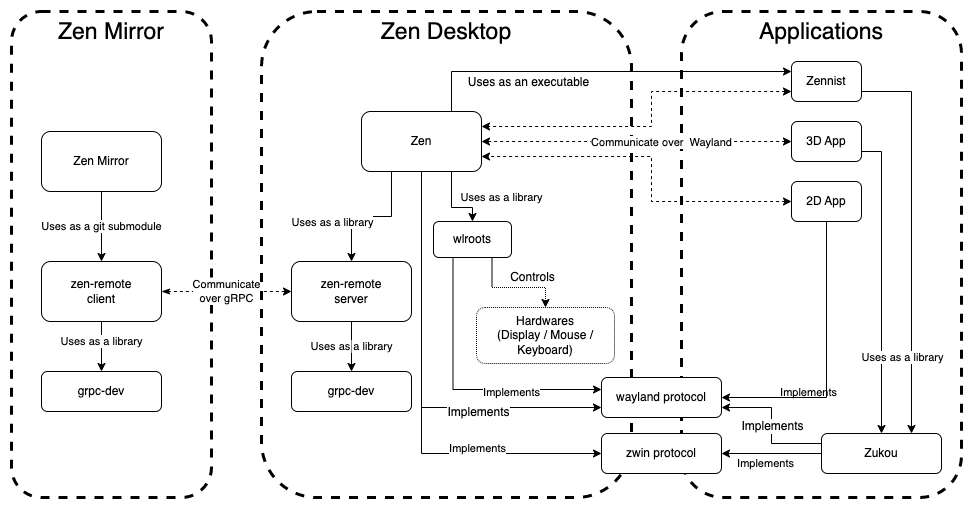
\includegraphics[keepaspectratio, width=\linewidth]{fig/development/overview.png}
  \caption{Zwinを構成するレポジトリとライブラリの関係を表した図.}
  \label{fig:overview}
\end{figure}

\subsection{Meta Quest 2への対応}

Meta Quest 2 はPCなどに接続することなく,単体でアプリケーションをインストールして利用できる
スタンドアローン型のヘッドセットである.
しかし本プロジェクトの要件として既存の2Dアプリケーションの利用が可能であり,
2Dディスプレイでのデスクトップ環境と行き来できる必要があるため,
PCに接続して利用することが求められる.

\subsubsection{既存技術の検討}
\label{subsubsection:exsiting-technology}

Meta Quest 2をPCに接続して利用するための技術としては主に以下のようなものがあるが,
それぞれに示した理由によって利用できなかった.

\begin{itemize}
  \item \textbf{Meta Quest Link}
        \footnote{Meta. "Meta Quest Link"
          \url{https://www.meta.com/ja-jp/help/quest/articles/headsets-and-accessories/oculus-link/}
          (accessed on 12 Feb. 2023)} \\
        Meta Quest LinkはPCを用いたVR環境(PCVR)のヘッドセットとして有線または無線でMeta Questを
        用いることができるようにする仕組みである.
        Zwinでは理想のWindowing Systemを自作するためにLinuxのみに対応しているが,
        Meta Quest LinkはWindowsのみに対応しているため,これを用いることはできなかった.
        Linux向けのMeta Quest Linkに相当するものを開発しているOSSなどもあるが,
        開発途中であったためZwinで用いるには十分でなかった.
  \item \textbf{ALVR}
        \footnote{alvr-org "ALVR GitBub repository". \url{https://github.com/alvr-org/ALVR} (accessed on 12 Feb. 2023)} \\
        ALVR は PCVR のヘッドセットとしてスタンドアローン型のヘッドセットを用いることが
        できるようする仕組みである.
        LinuxとOculus Questの組み合わせで動作するため当初はこれを用いる計画であった.
        しかし実装を進めていく中で,Zwinが2Dディスプレイ環境を同時に作っているという
        特殊な環境下であるために,技術的にALVRを利用するのは難しいという結論に至った.
\end{itemize}

\subsubsection{独自リモートレンダリングシステムの開発}

以上に示したとおり,既存技術では本プロジェクトに必要な条件を満たせていなかった.
また既存技術ではいずれも
OpenXR\footnote{The Khronos Group. "OpenXR overview" \url{https://www.khronos.org/openxr/} (accessed on 12 Feb. 2023)}
やOpenVR\footnote{Valve Corporation. "OpenVR" \url{https://partner.steamgames.com/doc/features/steamvr/openvr} (accessed on 12 Feb. 2023)}
といった,既存のAPIで開発された
アプリケーションをスタンドアローン型ヘッドセットで利用できる仕組みである.
そのため,アプリケーションがそれらのAPIを用いてレンダリングした結果のフレームバッファを
動画としてネットワーク越しに送るという手法をとっている.
ZwinではOpenXRのAPIを必ずしも用いる必要はなく,
独自のリモートレンダリングシステムをzen-remoteというライブラリとして実装した.
これによって以下のような利点を得ることができた.

\begin{itemize}
  \item レンダリングをMeta Quest側に任せることで,PC側に高いコンピューティングリソース
        を求める必要がなくなり,ラップトップPCでも動作させることができる.
        これによってさらに利用者の母数を増やすことができる.
  \item レンダリングをMeta Quest側に任せることで,レンダリングのために視点情報を
        ネットワーク越しにPCへ伝える必要がなくなり,より安定したレンダリングが可能になる.
  \item レンダリングに必要な情報の更新時のみネットワーク越しにデータを転送するため,
        毎フレームデータを転送する必要がなく,よりネットワーク帯域を節約できる.
\end{itemize}

\subsection{デスクトップ環境の実装}
期間中に行った,デスクトップ環境としての完成度向上の研究開発内容を以下に示す.

\subsubsection{2Dウィンドウの配置}
3Dアプリが少ない初期フェーズにおいては,既存の2D Wayland AppがVRで快適に使えることが重要なアピールポイントとなるので,2Dウィンドウの配置方法を検討した.

当初,VR内の2Dウィンドウの表示については,仮想的なモニターを3D空間に配置しその中に表示する案と,各ウィンドウを個別に3D空間内に配置する案があった.
仮想的なモニターではせっかくのVRの自由度を活かせない,しかし個別に3D空間に配置すると奥行方向の操作を各ウィンドウごとにする必要があり操作が非常に煩雑になる,というトレードオフを検討した結果,その中間案として「ボード」を採用した.
ボードは2Dウィンドウがスナップする面で,仮想モニターのように3D空間内に配置される.ウィンドウをあるボードから別のボードにドラッグして移動したり,ボード自体を自由に動かしたり削除・追加したりすることができる.仮想モニターの適度な制約による操作の手軽さと,VRならではの自由度を両立することを目指した.

\begin{figure}[htbp]
  \centering
  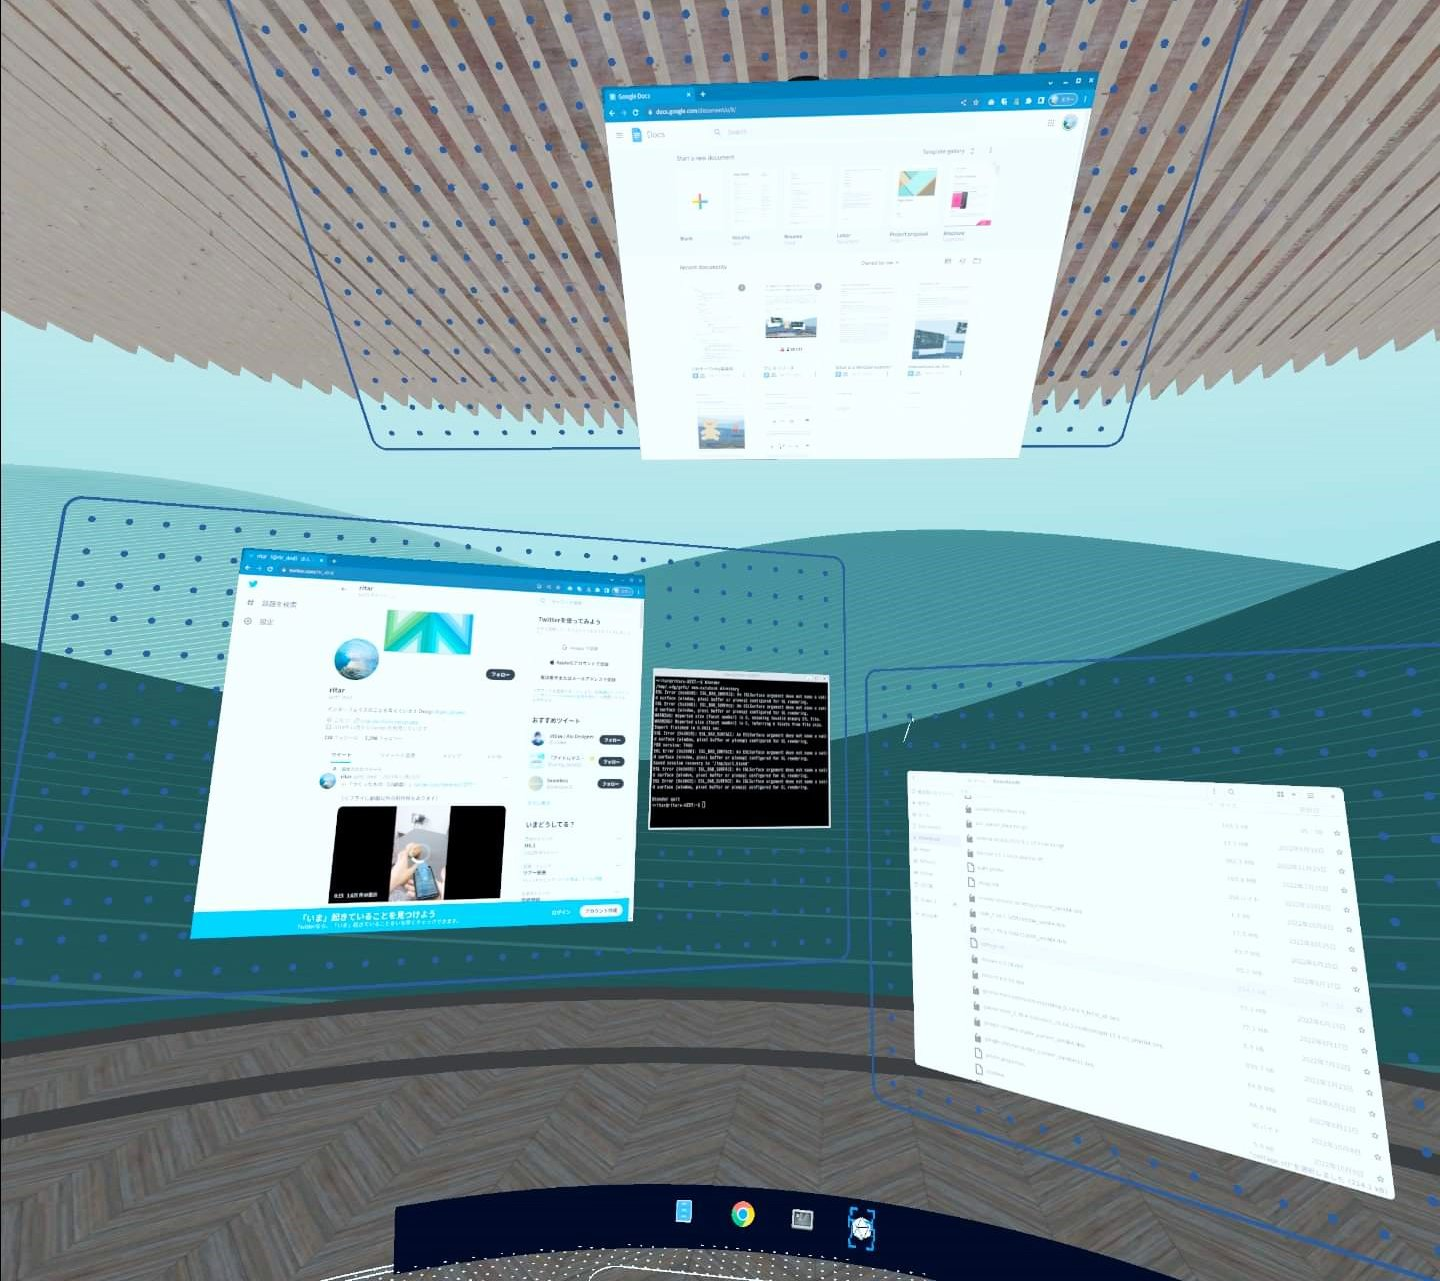
\includegraphics[keepaspectratio, width=0.7\linewidth]{fig/development/board-vr.jpeg}
  \caption{VRでボードに2Dウィンドウを表示している様子.}
  \label{fig:board-vr}
\end{figure}

\subsubsection{座標系とシート面}
2Dウィンドウと同様,各種3DアプリやボードをどのようにVR空間に配置・移動するかという問題があった.デスクトップ環境として2Dアプリを使った長時間の使用に耐えるため,Zwinではマウスとキーボードを入力デバイスとして採用している.マウスの2次元の動きをどのように3次元に変換するかが鍵となった.

様々なプロトタイプを開発し検討した結果,3DオブジェクトをVRに配置する際に求める配置方法は,以下の2つしかないのではないかという結論に至った.

\begin{itemize}
  \item \textbf{自分中心座標}(図\ref{fig:minority-report}) \\
        ユーザーの周辺に,常にユーザー側を向くようにアプリを配置する方法.
  \item \textbf{環境中心座標}(図\ref{fig:hololens}) \\
        環境の任意の場所に紐づけてアプリを配置する方法.
\end{itemize}

\begin{figure}[htbp]
  \begin{minipage}[b]{0.50\linewidth}
    \centering
    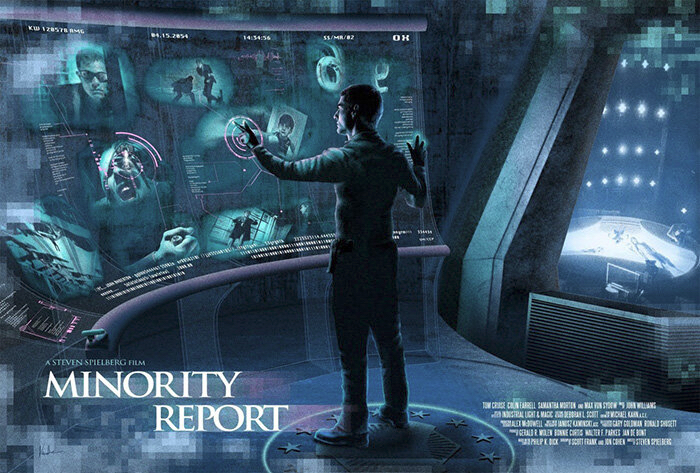
\includegraphics[keepaspectratio, width=\linewidth]{fig/development/minority-report.png}
    \caption{自分中心座標の例(映画『マイノリティ・リポート』に登場するインターフェイス\cite{minorityreport}).}
    \label{fig:minority-report}
  \end{minipage}
  \begin{minipage}[t]{0.50\linewidth}
    \centering
    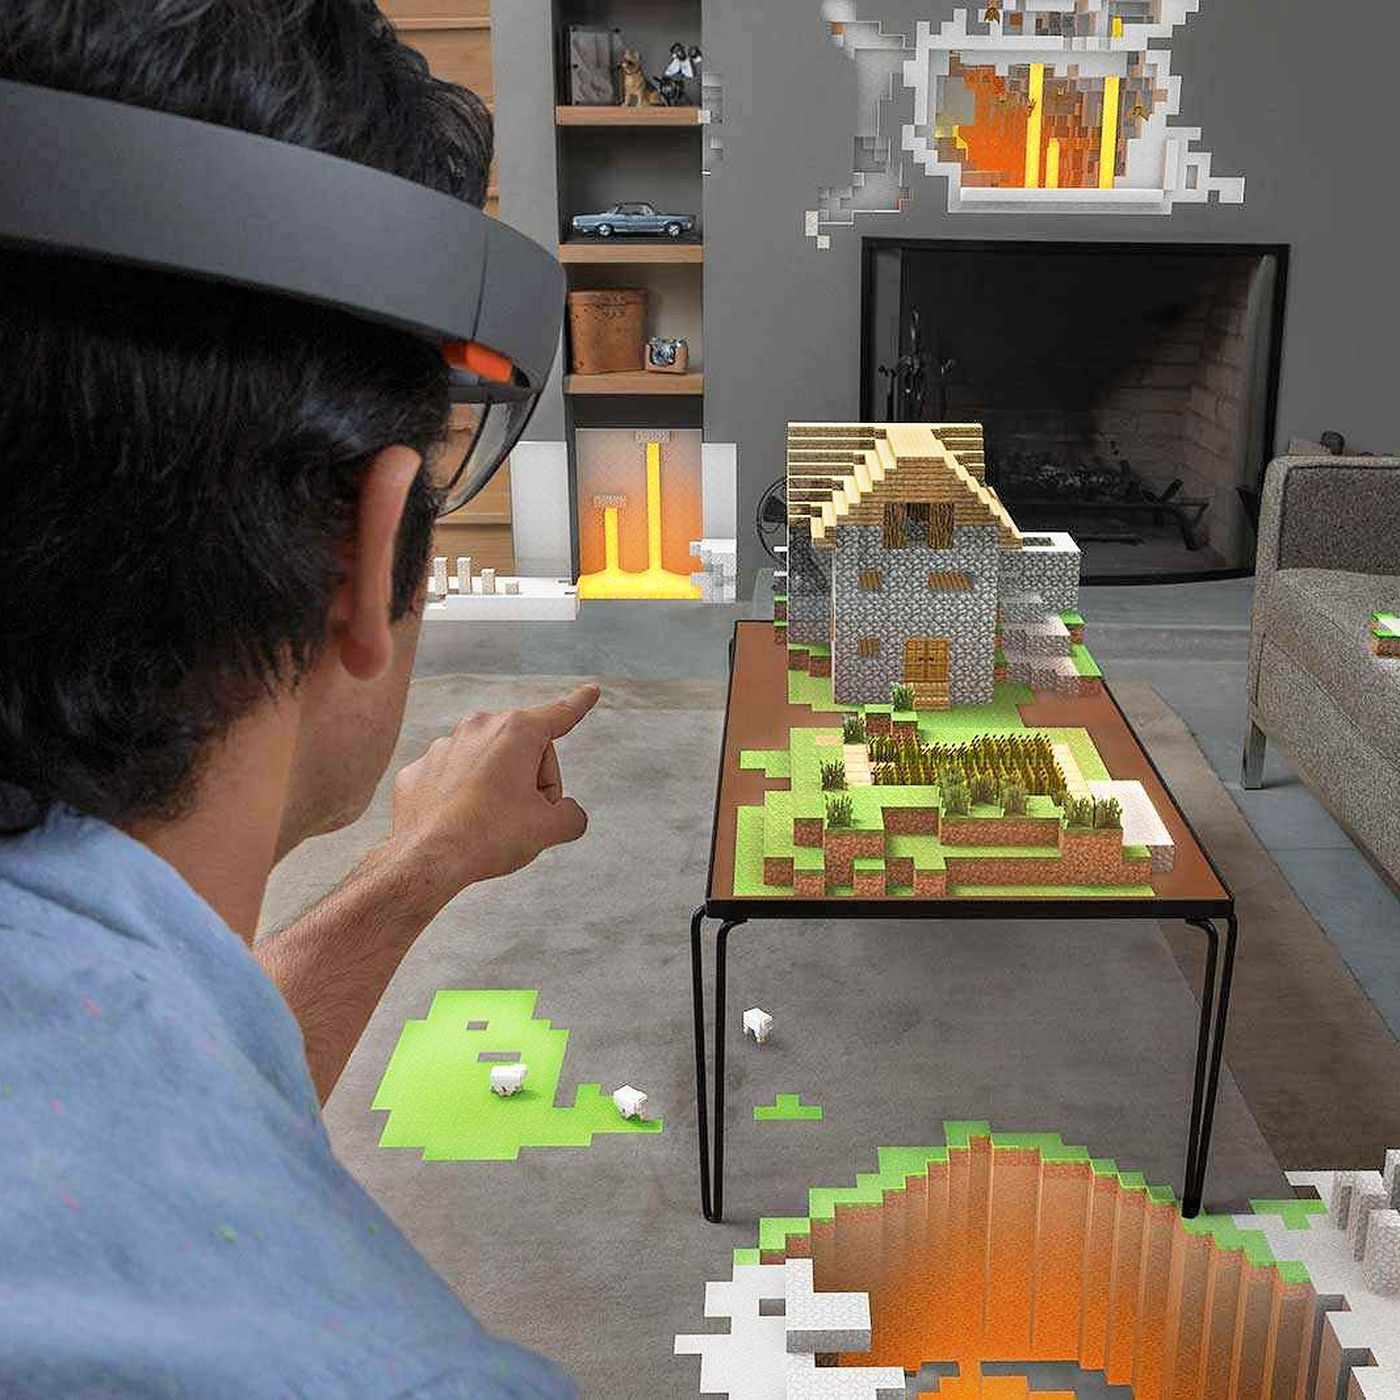
\includegraphics[keepaspectratio, width=0.7\linewidth]{fig/development/hololens.png}
    \caption{環境中心座標の例(Microsoft HoloLens 2\cite{hololens}).}
    \label{fig:hololens}
  \end{minipage}
\end{figure}

デスクトップ環境として,まずは自分中心座標での操作にフォーカスし,2Dウィンドウが快適に使える土壌が整った後に環境中心座標に対応していく方針とした.

自分中心座標において,アプリケーションはシート面(Seat capsule)という面に張り付いて移動することとした.
シート面はカプセルのような形状になっており,ユーザーの視線付近の高さでは円柱,それ以外の高さでは球面となっている(図\ref{fig:seat}).
これにより,ある程度の高さまでは垂直を保ったまま移動するので微妙な傾きに悩まされなくて済み,極端に上や下に配置した場合にはユーザ側を向くので可読性が確保できる.

\begin{figure}[htbp]
  \centering
  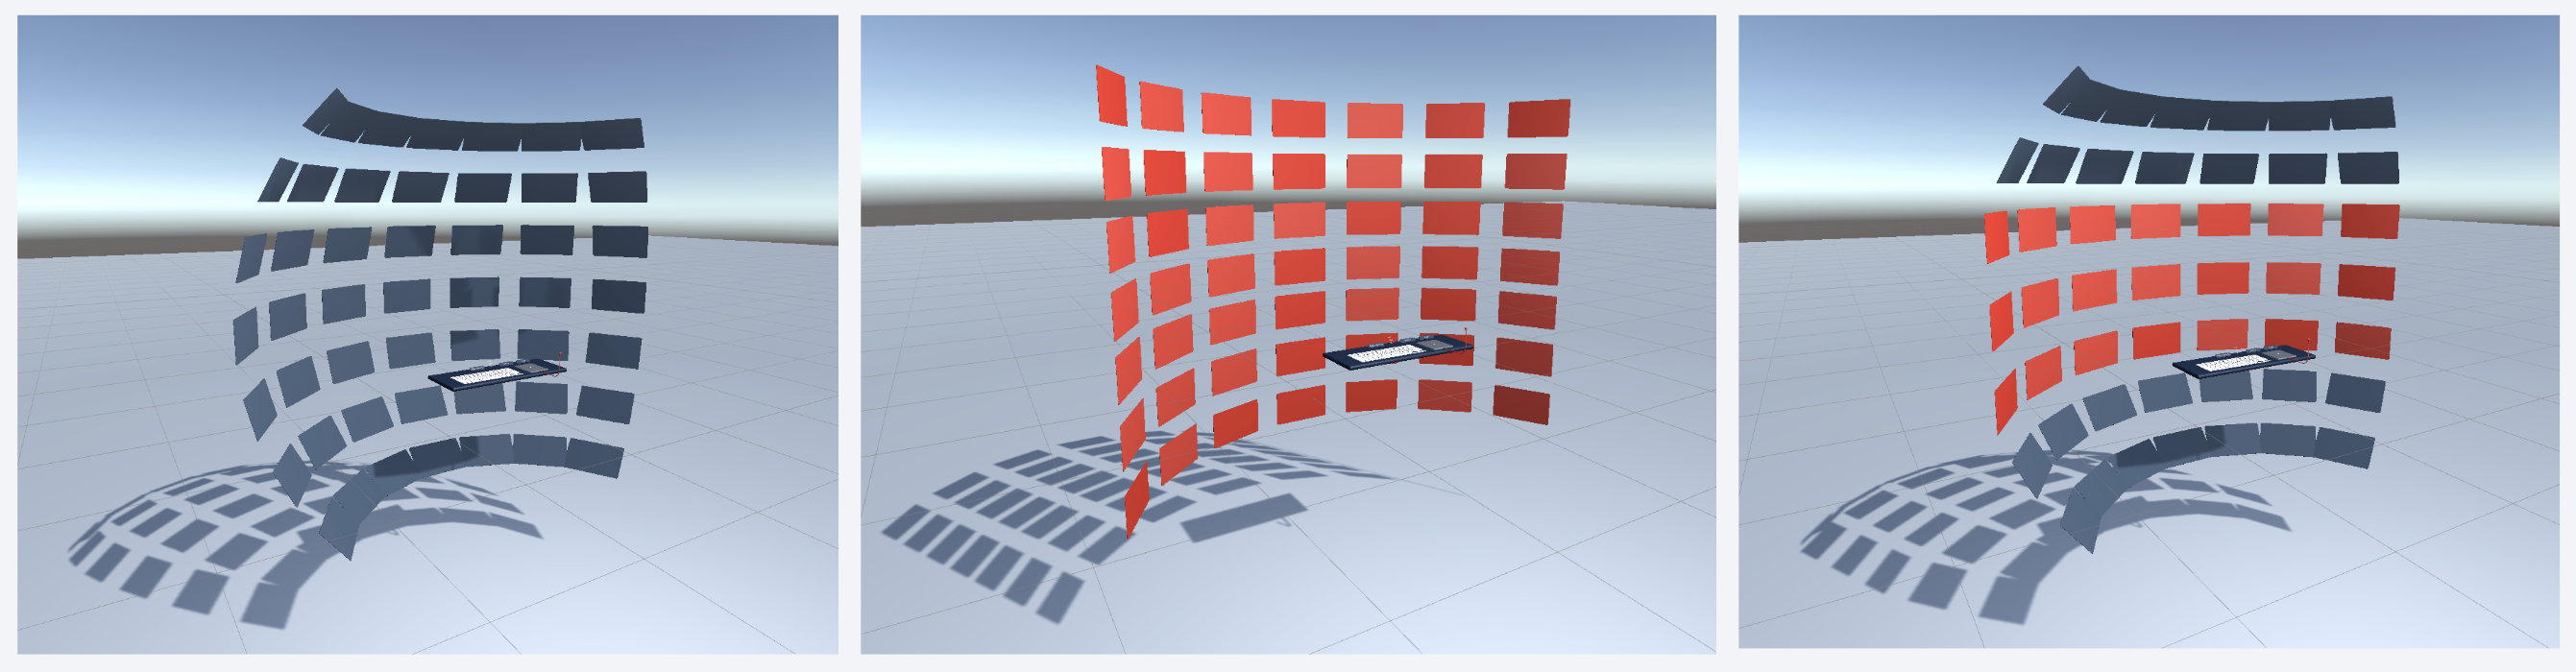
\includegraphics[keepaspectratio, width=0.9\linewidth]{fig/development/seat-capsule.png}
  \caption{ウィンドウの配置の模式図.左:極座標.中:円柱座標.右:実際に採用したシート面.}
  \label{fig:seat}
\end{figure}

自分中心座標へのフォーカス,ボードとシート面の導入により,2D入力デバイスであるマウスで快適にVR内の2D・3Dアプリを配置できるようになった.

\subsubsection{3D背景,机とランチャー}
VRのウィンドウシステムとして日常使いするために,心地よい環境と完結した機能が存在する必要がある.
新たにデザインしたデフォルトの3D背景は,VRならではの開放感と作業環境としての落ち着きを両立するため,天井と空が同時に見える設計,また落ち着いたカラーテーマとした(図\ref{fig:board-vr}).

さらに,自分が環境内にいるという感覚を得るためには,机がVRに表示されていることが重要だとわかり,透明な机を環境に配置した.机はシート面に沿った形状とし,自然な操作や水平感の把握の妨げにならないよう心がけた.
机には簡易的なアプリケーションランチャーを設置し,VR内で操作が完結するようにした.3Dアプリには3Dのアイコンを設定できる仕組みとした.

\subsubsection{文字サイズと可読性}
現状のVRヘッドセット内で2Dウィンドウを使うにあたり,最もクリティカルになるのが可読性である.
過去に競合のVRデスクトップを使ったことがあるユーザーにインタビューしたところ,使うのをやめた理由としてテキストの可読性が低いことを挙げたユーザーが多かった.

Zwinでは,Meta Quest 2でのテキストの可読性を検証し,テキストが読めることが確認できた距離・ウィンドウサイズをデフォルトとしている.また最大限テキストの可読性が上がるようアンチエイリアシングについても様々な検証を行った.

\subsubsection{サンプル3Dアプリ(3Dオブジェクトビューア)}
Zwinの3Dアプリの世界観を伝えるため,サンプルアプリとして3Dオブジェクトビューアを開発した(図\ref{fig:viewer}).
STLファイルを表示し,マウスのスクロール操作によって左右にオブジェクトを回転させることができる.
通常の2Dウィンドウのように,複数のウィンドウを開き3Dオブジェクトを見比べることが可能である.
ファイルエクスプローラでSTLファイルをダブルクリックすると,このアプリが開くように設定することができる.
慣れ親しんだ2Dウィンドウでの操作と同じ感覚で,3Dアプリを3Dのまま表示・使用できる,というZwinの特徴を最大限伝えられる設計とした.

\begin{figure}[htbp]
  \centering
  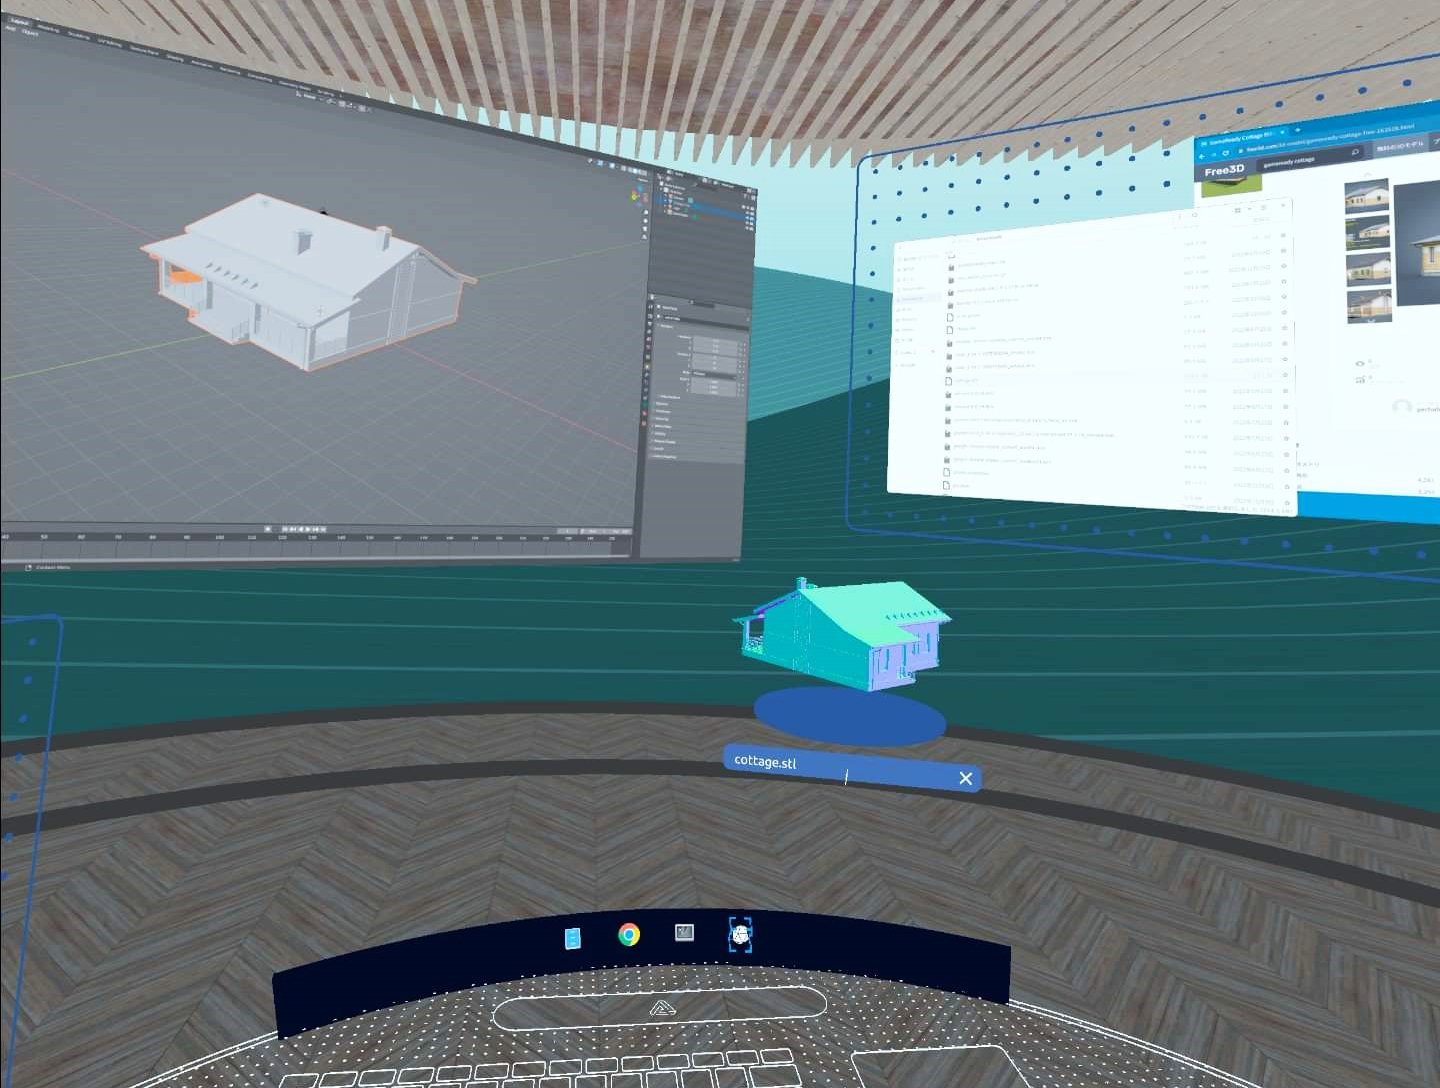
\includegraphics[keepaspectratio, width=0.7\linewidth]{fig/development/viewer.png}
  \caption{3DオブジェクトビューアをBlender・Chromeとともに開いている様子.}
  \label{fig:viewer}
\end{figure}


\subsection{2Dデスクトップ環境との統合}

Zwinでは2Dのデスクトップ環境とXR空間でのデスクトップ環境との間をシームレスに
移動できることを目指した.

ディスプレイを全く必要とせず,PCとヘッドセットだけで完結するシステムも
考えられるが,長時間ヘッドセットを装着して作業することは負担が大きい点や,
技術的に2Dのデスクトップ環境を用意しなければヘッドセットをセットアップするための
アプリケーションなどがそもそも表示できないため,
XR環境を使い始めることが難しいという点から2Dデスクトップ環境を用いることにした.

\subsubsection{2Dデスクトップ環境の実装}

2Dデスクトップ環境に一般的な以下の機能を実装した.

\begin{itemize}
  \item Wayland アプリケーションやポップアップの表示
  \item Wayland アプリケーションの移動やリサイズ,最大化の実装
  \item キーボードやポインタなどの入力の伝達
  \item アプリケーションランチャー
  \item ログアウトボタン
  \item バーチャルデスクトップ(詳しくは\ref{subsubsection:2d-board}で述べる)
  \item 背景画像やランチャーに表示するアプリケーションの設定機能
\end{itemize}

これに加えて,XR空間での利用を可能にするため以下の実装をした.

\begin{itemize}
  \item 利用可能なヘッドセット一覧とXRモードへの移行ボタン
  \item XRモードの時に2Dディスプレイに表示する案内画面
  \item Wayland アプリケーションのコンテンツをXR空間に表示するため,
        バッファとして取り出し可能にするためのwlrootsのレンダラー部分の拡張実装
\end{itemize}

\subsubsection{2Dでのボード}
\label{subsubsection:2d-board}

VRにおいて2Dウィンドウの操作を簡便にするために導入したボードだが,2Dスクリーンにおいては,2Dデスクトップ環境で一般的な「バーチャルデスクトップ」の役割を果たす.
2Dデスクトップにおけるバーチャルデスクトップとは,ウィンドウをいくつもまとめた「デスクトップ」を複数切り替え可能にするという仕組みである.
Zenでは,ボード一覧を下部のタスクバーにまとめ,どのボードをスクリーンに表示するかを切り替え可能にすることで,ボードをバーチャルデスクトップとして用いることができる(図\ref{fig:board-2d}).
2Dデスクトップ環境とXR環境とを切り替える際には,ボードに割り当てられたウィンドウやその位置といった
状態は保存されるため,ユーザーはシームレスに作業を続けることができる.

\begin{figure}[htbp]
  \centering
  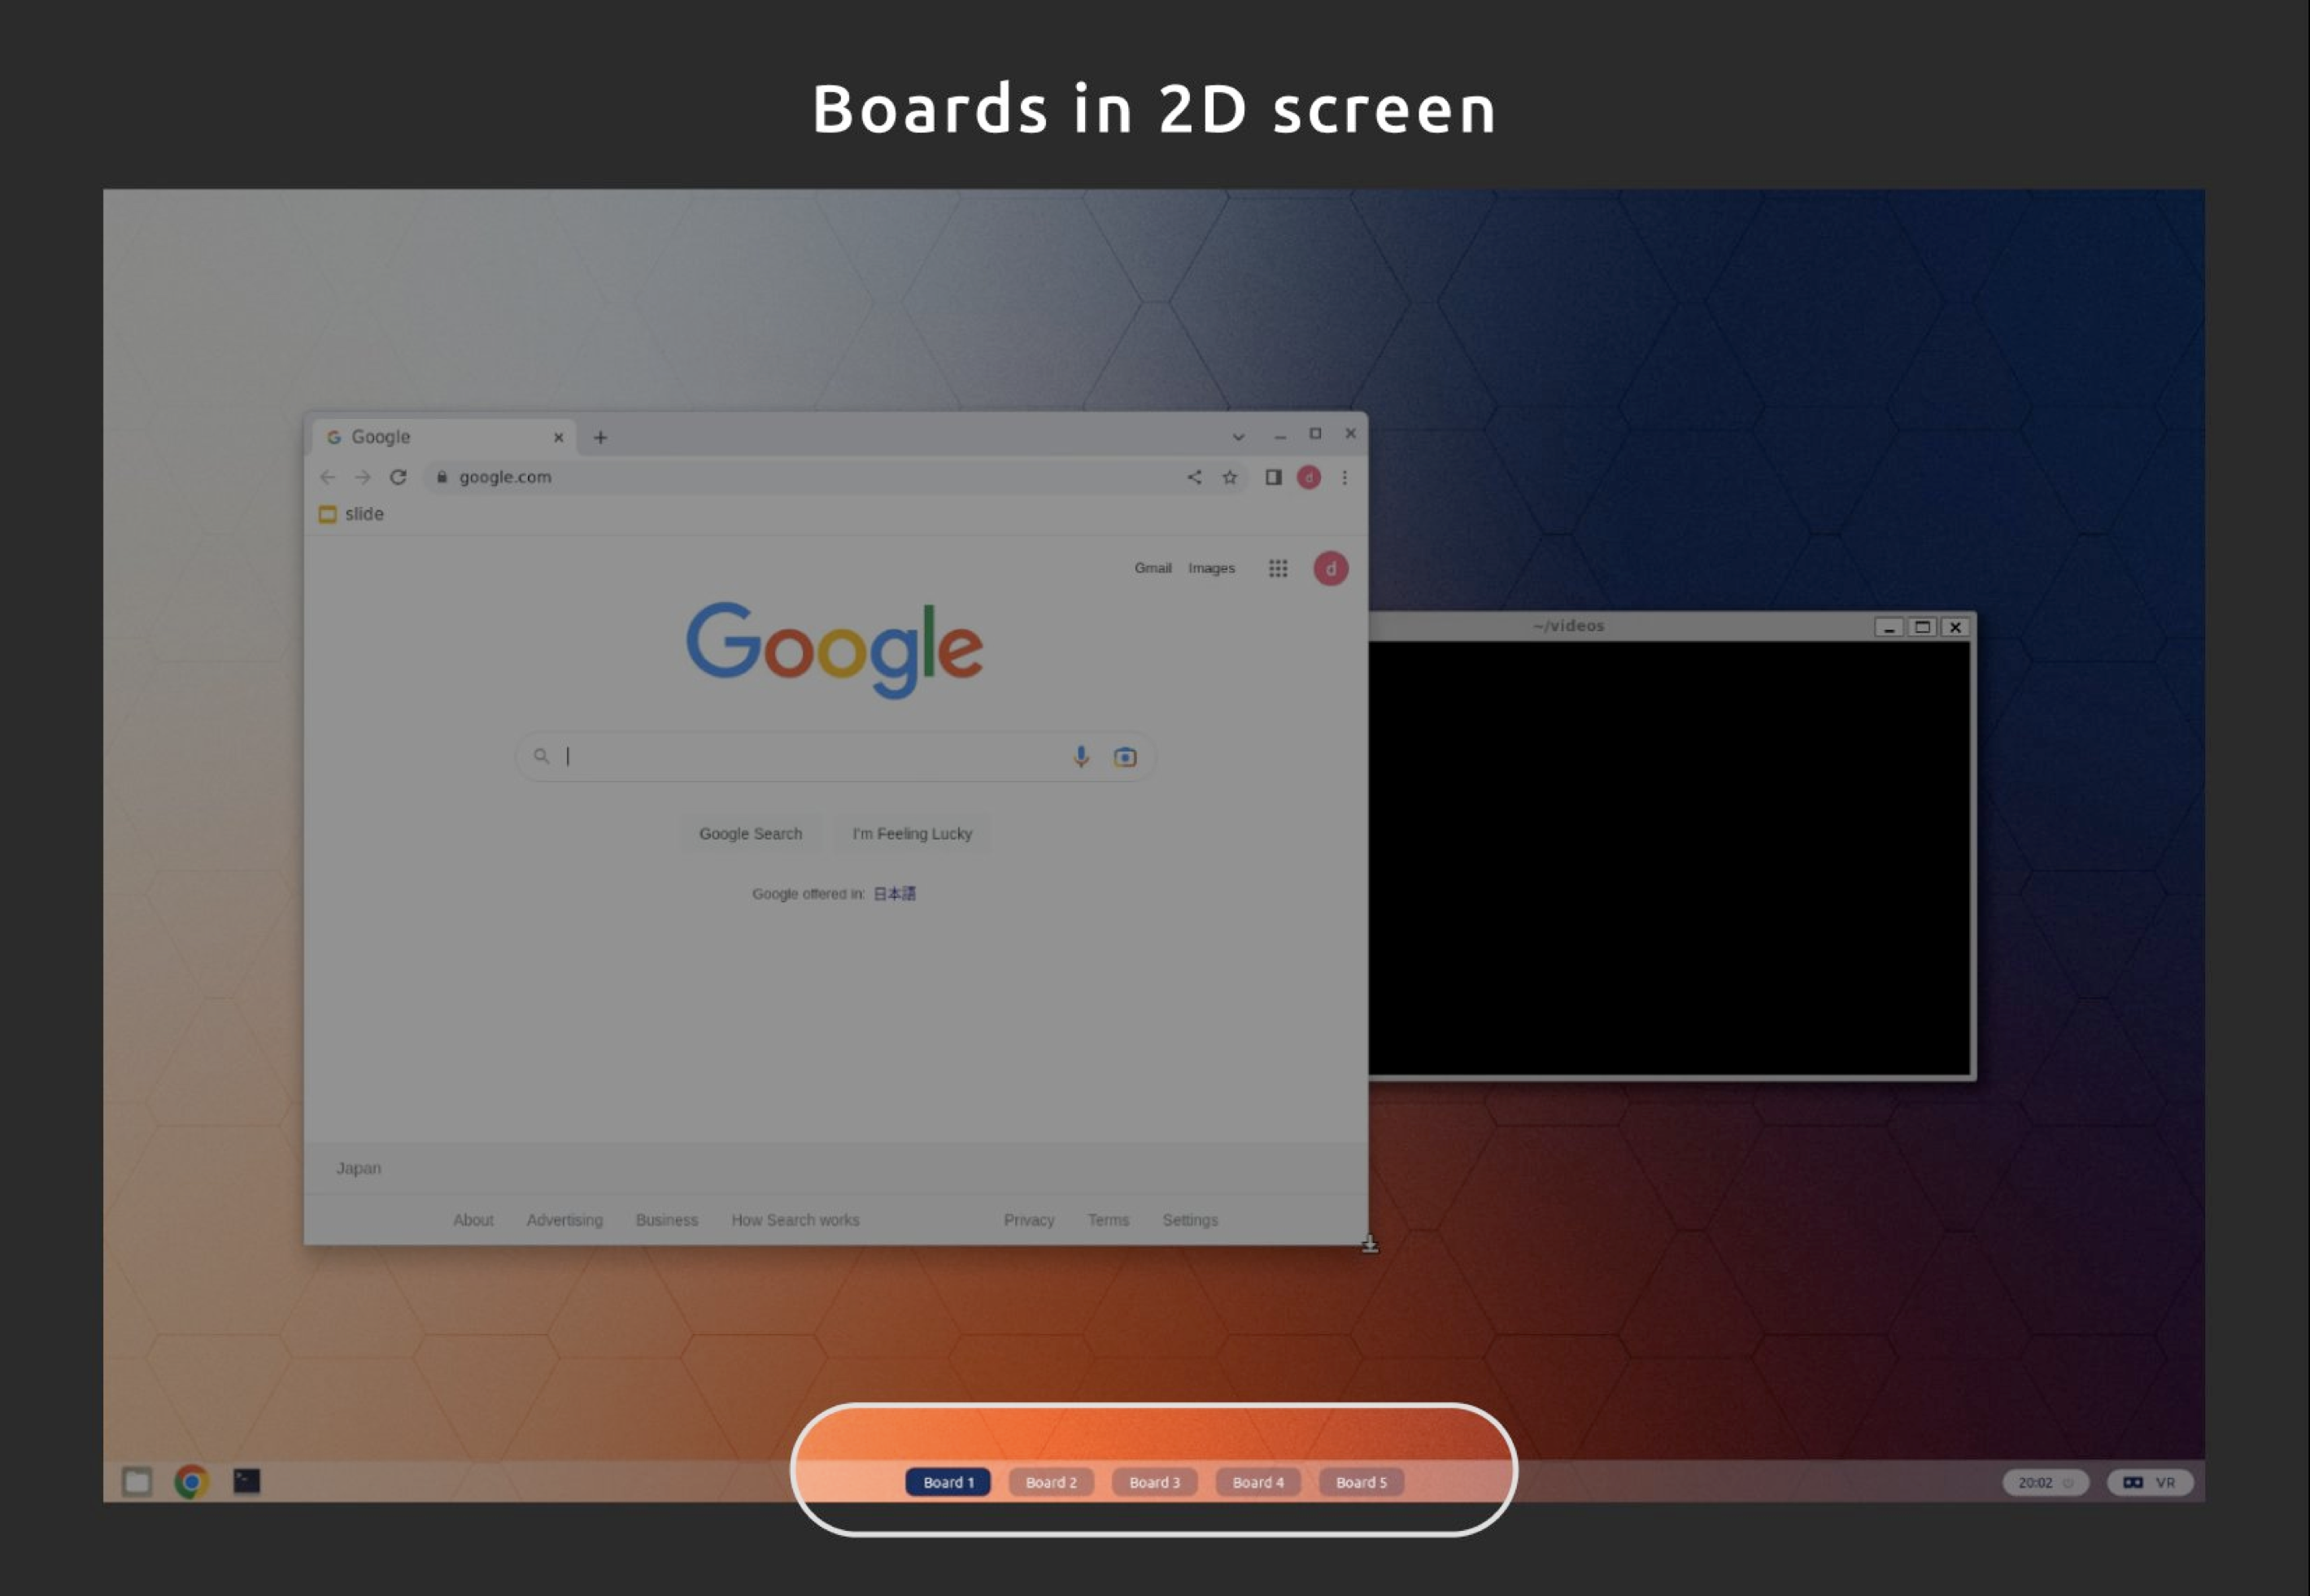
\includegraphics[keepaspectratio, width=0.7\linewidth]{fig/development/board-2d.png}
  \caption{2D画面におけるボード.}
  \label{fig:board-2d}
\end{figure}

% \begin{enumerate}
%   \item 使用フローを一通り解説,接続についてとか
%   \item 2DでのBoardについて
% \end{enumerate}
